

\section{Experiments - Installations}
In Section \ref{transformer-intro} above the workings of a Transformer and the workings of Generative Pre-training Transformer 2 are described. It is proposed there that they are similar. For the experiments section they are totally separate.

There are several basic neural network models. One is the basic Sequence to Sequence GRU model typically used for neural machine translation. There are also two Transformers and the Generative Pre-training Transformer 2. We try to touch on each model type and also distinguish between chatbot operation and smart-speaker operation. 

There are only three Raspberry Pi boards. There is also a Jetson Nano board. Installation of all four models is attempted on Pi boards, but only three Raspberry Pi installations are kept. The Nano is used for an additional GPT2 installation and serves as a speed comparison with the Raspberry Pi. 

The model that did not make it to permanent installation on a Raspberry Pi was the smaller Transformer with the Persona corpus. There are four complete installations with the inclusion of the Nano board.

\subsection{Questions}
Below is a list of questions asked of all models. From this list and the answers from each model we try to make comparisons between the models about their strengths.

\begin{verbatim}
Hello.
What is your name? 
What time is it?
What do you do?
What is your favorite color?
Do you like red?
Do you like blue?
What is your favorite candy?
Do you like ice cream?
Good bye.
\end{verbatim}

Without considering reply time, the GPT2 model worked best. 

Subjectively the first Transformer model with the Persona corpus did not perform as well as the Generative Pre-training Transformer 2 model. It did not perform better than the Gated Recurrent Unit model either. 

The model from the Gated Recurrent Unit tutorial performed well. It was better than the initial Transformer model and on par with the larger Transformer model. It was not better than the Generative Pre-training Transformer 2.

We visit and revisit this checklist to subjectively rate our chatbots.

%\noindent \textbf{Checklist:}
\subsection{Checklist} 

\begin{itemize}
	
	\item [1.] Are all the responses are in plain English? Are any of the answers gibberish?
	
	\item [2.] Is there a  variety of answers? Are all answers the same?
	
	\item [3.] Does the model give good answers to the questions about `favorite color' and `favorite candy'? The model could have a set of easy answers that it can use for this kind of question or it considers the question separately. 
	
	\item [4.] `No' is a safe answer for many types of question as it is clearly English, it follows logically, and it is short and easy to remember. Another safe answer is `I don't know'. Does the model use these answer at all times?
	
	\item [5.] Does the model answer well to `Hello' and `Good bye'?
	
\end{itemize}

The reason for question 1, 2 and 5 are straight forward. The reason for question 3 is to determine how well the model understands English. If the answers to `favorite candy' and `favorite color' are the same, then the model is pretty simple. If the answers are different then the answer set that the model uses is larger. The model might or might not know there is a difference to candy and color. %This is just one example of the model being larger. 

A simpler model will answer `I don't know' for the `favorite candy' and `favorite color' questions. It can even answer questions like `do you like red' and `do you like ice cream' with `I don't know'. 

Question 4 refers to weather simple `No' answers are used all the time to answer questions that would otherwise need complex sentence structure. A simpler model might figure out during training that `No' answers were easier to remember and could be applied in many places.

\section{Chatbot - Gated Recurrent Unit Model}
We have two models based on the sequnce to sequence architecture proposed by Vinyals et al \cite{DBLP:journals/corr/VinyalsL15}. One model was largely written by hand. This first model does not work very well. The second model was taken largely from an online tutorial by  Inkawhich et al \cite{2018Inkawhich}.

We trained this sequence to sequence model on a large english corpus in an attempt to produce a chatbot. This model does not use a Transformer architecture.

This second sequence to sequence model from the GRU tutorial performed exactly as expected. It answered a number of subjective questions with original, authentic answers. Almost all the answers made sense in the English language.

\subsection{Questions}
This is the sample question list as it was answered by the GRU model.

%\begin{minipage}{2in}
\begin{verbatim}
> hello .
you re a good man .
> what is your name ?
smith .
> what time is it ?
i don t know .
> what do you do ?
i m a comedian .
> what is your favorite color ?
i don t know .
> do you like red ?
no .
> do you like blue ?
no .
> what is your favorite candy ?
it s a big one .
> do you like ice cream ?
no .
> good bye .
good bye .
\end{verbatim}
%\end{minipage}
%\bigskip


%\noindent \textbf{Checklist:} 
\subsection{Checklist}

\begin{itemize}
	\item [1.] \textbf{Are all the responses are in plain English? Are any of the answers gibberish?}
	
	\item [] All the responses are in plain English. There is no gibberish.
	
	\item [2.] \textbf{Is there a  variety of answers? Are all answers the same?}
	
	\item [] Not all answers are the same.
	\item [3.] \textbf{Does the model give good answers to the questions about `favorite color' and `favorite candy'? The model could have a set of easy answers that it can use for this kind of question or it considers the question separately.} 
	
	\item[] It is debatable weather or not the answers to the questions about `favorite color' and `favorite candy' are good. It is good that the two types of questions don't have the same answers.
	
	\item [4.] \textbf{`No' is a safe answer for many types of question as it is clearly English, it follows logically, and it is short and easy to remember. Another safe answer is `I don't know'. Does the model use these answer at all times?}
	
	\item[] This model uses that answer at times. It does not use `no' always.
	
	\item [5.] \textbf{Does the model answer well to `Hello' and `Good bye'?}
	
	\item []The model answers well to `Hello' and `Good bye'.
\end{itemize}

This is a reasonably good model. It is also very light weight.

\section{Smart Speaker - Gated Recurrent Unit Model}

The Gated Recurrent Unit model was installed on a Raspberry Pi. This allowed us to test out speech-to-text and text-to-speech libraries. The Raspberry Pi model was 3B. The RAM requirements were less than 500MB and the trained model answered questions on the Raspberry Pi almost instantaneously.

For this experiment we compiled the Pytorch library for Raspberry Pi.

The Raspberry Pi was outfitted with a microphone and a speaker and nothing more. It was also configured so that the Pytorch sequence to sequence model ran automatically on startup.

The model requires access to the internet for the exchange that the speech to text software has to make with the Google servers. If there is no internet the model doesn't work.

As there was no monitor and it took some time for the model to launch, the program was coded to beep when the model was ready to accept input. At that point the model beeps once.

\section{Chatbot - Transformer Model with Persona Corpus}
Using the Persona corpus we trained a Transformer model to use as a chatbot. This Transformer was not pre-trained with any large corpus, so this example did not use transfer learning. The Persona corpus comes from Mazar{\'{e}} et al \cite{DBLP:journals/corr/abs-1809-01984}.

This model uses the tensorflow library, not Pytorch, and a Transformer model that is somewhat small. The model has encoder and decoder sections. The model uses 2 layers, 4 heads, and a hidden size of 128.

The memory footprint of the model while it was running was below 1 Gigabyte. It is conceivable that the model could be installed on a Raspberry Pi board. That requires a python package called `tensorflow-model-server' and this package had to be provided for ARMv7 for the Raspberry Pi. 

\subsection{Training}
First the model was trained on the persona corpus until a familiar pattern emerged. When the model began to answer all questions with the phrase "I don't know" training was stopped. 

At that time the corpus was modified to include no sentences that have the word "don't" in them. Training was started again until the output contained nothing but the phrase "I'm sorry." 

At that time the corpus was modified to include no sentences that have the word "sorry" in them. Training was started again and was continued for some period. A further segment of training was not attempted. 

At this point, after looking at the change in loss, further training was not thought of as helpful. Loss stopped improving at some point in this process, and this lack of improvement was taken as a sign that further progress was not likely.

\subsection{Questions}
Subjectively this Transformer model is not better than the original Gated Recurrent Unit model from the Sequence to sequence tutorial. It can respond to something like four sentences. When it comes upon a question that it doesn't expect it defaults to a certain sentence. It can answer questions that you might ask in a rudimentary conversation. It has answers to prompts like `hi', `How are you?' and `What do you do?'. If you tell it your name it will tell you that its name is `Sarah'. It doesn't answer arbitrary questions. It cannot answer 'What is your favorite color?'. It can not tell you the time. The default reply sentence for unknown prompts is `Hi, how are you today?'

This is the sample question list as it was answered by the model.

\begin{verbatim}
> hello
hi , how are you today ?
> what is your name?
hi , how are you today ?
> what time is it ?
I like to read a lot
> what do you do ?
i'm a student
> what is your favorite color ?
hi , how are you today ?
> do you like red ?
hi , how are you today ?
> do you like blue ?
hi , how are you today ?
> what is your favorite candy ?
hi , how are you today ?
> do you like ice cream ?
yes , i do 
> good bye
hi , how are you today ?
\end{verbatim}

%\noindent \textbf{Checklist:} 
\subsection{Checklist}

\begin{itemize}
	\item [1.] \textbf{Are all the responses are in plain English? Are any of the answers gibberish?}
	
	\item []All the responses are in plain English. There is no gibberish.
	
	\item [2.] \textbf{Is there a  variety of answers? Are all answers the same?}
	
	\item []There is a variety of answers. There is not a great variety though, and this is a problem for this model.
	
	\item [3.] \textbf{Does the model give good answers to the questions about `favorite color' and `favorite candy'? The model could have a set of easy answers that it can use for this kind of question or it considers the question separately.} 
	
	\item []Some of the answers are re-used and do not follow logically from the questions. The `favorite color' and `favorite candy' questions are nearly ignored. For those questions the model answers with `Hi, how are you today?'. This seems to be the model's default answer.
	
	\item [4.] \textbf{`No' is a safe answer for many types of question as it is clearly English, it follows logically, and it is short and easy to remember. Another safe answer is `I don't know'. Does the model use these answer at all times?}
	
	\item []The model does not use `No' or `I don't know'.
	
	\item [5.] \textbf{Does the model answer well to `Hello' and `Good bye'?}
	
	\item []The model does not have an answer for `Good bye'. It does answer for `Hello'.
	
\end{itemize}

This is a poor model. It does use English language answers, but does not perform well in many other respects.

\section{Smart Speaker - Transformer Model with Persona Corpus}

This Transformer model was tested on the Raspberry Pi. The model is not more dynamic than the GRU tutorial model. 

The Transformer model takes about two minutes to boot on the Raspberry Pi. After that the time between responses is slow. The time between the first two or three responses is uncomfortably slow. After those first responses the time between answers gets to be more natural.

There is one special tone that the Raspberry Pi gives at the end of loading the model. This tone notifies the user that the model is loaded and ready to respond to questions.

The Persona corpus model is not interesting to watch. Though smart speaker installation was attempted and ultimately successful, the Raspberry Pi that was used was required for another model. That other model worked better and was retained for the thesis.

\section{Chatbot - Transformer Model with Movie Corpus}


Using the Movie corpus we trained a Transformer model to use as a chatbot. This Transformer was not pre-trained with any large corpus, so this example did not use transfer learning. 

This is the model we refer to as the larger Transformer model. It is larger than the Transformer model with the Persona corpus but it is smaller than the smallest GPT2 model.

This model uses the Tensorflow library, not Pytorch. %, and a Transformer model that is larger than the other Transformer based model that uses the Persona corpus.

In contrast the Persona corpus model uses 2 layers, 4 heads, and a hidden size of 128. The Movie corpus model uses 6 layers, 8 heads, and a hidden size of 512. This model has both encoder and decoder sections.

The memory footprint of the Movie corpus model while it was running was above 1.5 Gigabyte. The model could be installed on a Raspberry Pi 4B board but it requires a python package called `tensorflow-model-server' and this package had to be built from source or somehow provided for the Raspberry Pi. 

The model was trained on the development computer in a x86\_64 environment. The model took about seven days to train with a CPU based processor. The goal for training was 50,000 lines from the movie corpus. After training the loss graph was consulted and the installed version was culled from the saved checkpoint at the 45,000 line point.


\begin{figure}[H]
	\begin{center}
		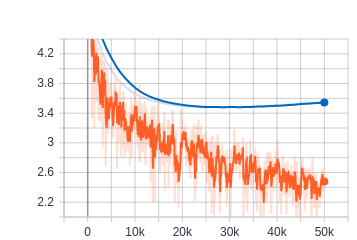
\includegraphics[scale=3.5]{Figure_2}
		
		
	\end{center}
	\caption[Loss - Larger Transformer Model]{Loss - Orange is training loss and blue is evaluation loss.}
	
	%\addcontentsline{lof}{section}{Word Embeddings}
\end{figure}

Subjectively this Transformer model is better than the Transformer model based on the smaller hyper-parameter set and the Persona Corpus.


%\begin{lstlisting}[language=bash]
\subsection{Questions}
This is the sample question list as it was answered by the model.

\begin{verbatim}
> Hello.
hello 
> What is your name?
i don't know 
> What time is it?
i don't know 
> What do you do?
what do you mean ?
> What is your favorite color?
i don't know 
> Do you like red?
no 
> Do you like blue?
yeah 
> What is your favorite candy?
i don't know 
> Do you like ice cream?
yeah 
> Good bye.
bye 
\end{verbatim}

%\noindent \textbf{Checklist:} 
\subsection{Checklist}

\begin{itemize}
	\item [1.] \textbf{Are all the responses are in plain English? Are any of the answers gibberish?}
	
	\item []All the responses are in plain English. 
	
	\item [2.] \textbf{Is there a  variety of answers? Are all answers the same?}
	
	\item []There is a variety of answers. 
	
	\item [3.] \textbf{Does the model give good answers to the questions about `favorite color' and `favorite candy'? The model could have a set of easy answers that it can use for this kind of question or it considers the question separately. }
	
	\item []The `favorite color' and `favorite candy' questions are ignored. The model does not have original answers for these questions. It will reply with `I don't know'.
	
	\item [4.] \textbf{`No' is a safe answer for many types of question as it is clearly English, it follows logically, and it is short and easy to remember. Another safe answer is `I don't know'. Does the model use these answer at all times?}
	
	\item []The model does in fact use `No' or `I don't know'. It does not use these exclusively.
	
	\item [5.] \textbf{Does the model answer well to `Hello' and `Good bye'?}
	
	\item []The model does have an answer for `Hello' and `Good bye'.
\end{itemize}

This is a reasonably good model. We prefer this model over the one that uses the Persona corpus.

\section{Smart Speaker - Transformer Model with Movie Corpus}

The Transformer model is installed on the Raspberry Pi. It takes about 6 seconds to answer any question.

The Transformer model takes about two minutes to boot on the Raspberry Pi. After that the time between responses is slow. 

There is a special tone that the Raspberry Pi gives at the end of loading the model. This tone notifies the user that the model is loaded and ready to respond to questions. The model is also configured to beep intermittently during operation to signal that it is processing an input. This is helpful for a configuration where there is no monitor.

A set of LED lights is installed on the Raspberry Pi to show when the model is processing input and when the model can take new input. The lights are helpful.


\section{Chatbot - Generative Pre-training Transformer 2 Model}

\label{install-gpt2-chatbot}
We used a pre-trained Generative Pre-training Transformer 2 model with the large english corpus to produce a chatbot and ascertain if this model works better than the sequence-to-sequence model. In our tests this worked well and this model was considered superior. The corpus is called `WebText'. We did not train this model ourselves.

For our experiments the Generative Pre-training Transformer 2 was used for the chatbot model in `zero-shot' mode. This means we did no special fine-tuning of the model in the application.

We did do some special coding for the input and output code in order to operate it as a chatbot. Output was limited to about 25 tokens. 

Input to the model was prepended with the character string "Q:" by our code. Output was observed to have the character string "A:" prepended to it. We assume therefore that the model was at some point exposed to the "Question/Answer" paradigm in written passages during its training. This was helpful.

Output from the model was usually larger in size than we needed. Also, output had the character of having some sensible utterance followed by some output that was only a partial sentence.

It was necessary to process the output. First the output was checked for the "A:" character string at the start. If it was there it was removed. Then the first complete sentence was used as output, while words and phrases after that were discarded.

\subsection{Context Experiment}
We decided that we would attempt to give the model some details that it could draw on during normal execution. We had two choices here. One choice was to train the model using fine-tuning and transfer learning to recognize certain questions and to supply answers. The other choice was to simply show the model the list of facts that we thought were important before every input sequence. This information would be summarized with each reply.

The second choice was more interesting. The text that the model was shown always included the name of the model (picked somewhat arbitrarily) along with information about the location of the model and the occupation. The time was also included.

This worked under most circumstances. Occasionally the model would report the wrong time when asked. This sort of activity is mysterious.

\subsection{History Experiment}
We tried concatenating all input and output and including it with each question. The hope was that the model would treat the `Q' and `A' as historical input and then it could refer to that input as it answered new questions. This didn't always work as expected. Sometimes the model was confused by the extra input. Sometimes it seemed to have no effect at all.

Without some mechanism of this sort the model has no notion of temporal context. The answers to questions could never possibly depend on the answers to past questions. Though this historical input did not always work, we retain the code in the hopes that at some point it is useful.

Consider the questions below.
\begin{verbatim}
> Do you like the color red?
I like the color red.
> What is your favorite color?
Red.
\end{verbatim}

\label{install-gpt2-history}

We like this output. The model is asked about the color `red'. Doing so the model is encouraged to pick `red' as the answer to the next question about color. When `favorite color' is requested, `red' is the answer. Without any history the model will answer the `favorite color' question with another answer. It may answer `pink' or it may answer `the colors of the rainbow'. 

From one sentence to the next the model is keeping track of the context of the conversation. History is considered. Unfortunately the results of our history experiment are not so robust. It is not always the case that the model chooses the color recently discussed as the `favorite' color.

\subsection{Artificial Intelligence Markup Language Experiment}
Tests showed that the Generative Pre-training Transformer 2 chatbot worked well. We wanted to continue and allow the chatbot to have more of the abilities of a smart speaker. We constructed a simple corpus that contained key phrases that we wanted the chatbot to recognize and act upon. We did some transfer learning with this new corpus.

We found that one of two things would happen. The chatbot would either learn the new phrases and forget all it's pre-training, or it would not learn the new phrases and it would retain all it's pre-training. For our examples there seemed to be no middle ground. Comparisons were made with all available models and a version without the transfer learning was settled on.

It was deemed helpful if the model could be given a question and instructed exactly how to answer it. To this end AIML files were constructed and an AIML kernel was employed. The user's question was shown to the AIML kernel and then the model was shown the kernel's output (if there was one) along with the original question. The hope was that the output could be controlled by the AIML component. 

At first it didn't work. The AIML confused the model, and the model would not reliably choose to answer with the AIML text, as it might with the time of day.

Later the AIML was modified to appear to the model with the `Q:' and `A:' at the beginning of the lines. Some of the time the model answered with the AIML. 

\subsection{Program Launching}

We did some programming that allowed the model to launch programs when directed to by the user. In this way we have tried to move our project closer to the smart-speakers that are produced commercially. The programming did not rely on the neural-network aspects of the model. Instead the code used string manipulation and simple word recognition. This code can be enabled when the model is run from the command line. This was not enabled for the Raspberry Pi.

There is no space prohibition for using the Program Launching code on the Raspberry Pi. Future work may use Chromecast as a way to connect the Raspberry Pi with the user's home TV or monitor. 

\subsection{Overall}

Subjectively the model was the best of those tested. The model would answer questions about it's location, it's name, and the time, faithfully most of the time. Interestingly there where times when it did not do so. Some times it used alternative answers. For example, it would answer with the time but not the correct time. This was odd.

Under almost all circumstances the output was sensible English. There were no times where the model replied with gibberish. 

The subject matter of the prompts did not need to be the same as the simple introductory conversation of the Transformer model. In fact any subject matter could be chosen and the model would answer. The model did not remember its own answers but it was consistent. Questions it answered include `What is your favorite color?' and `Do you like lollipops?'. 

\subsection{Questions}
This is the sample question list as it was answered by the model. Note that the information mentioned in the answer about the time was accurate when the test was run.

\begin{verbatim}
> hello
Hello.
> what is your name ?
My name is Jane.
> what time is it ?
02:59 PM January 28, 2020.
> what do you do ?
I am a student.
> what is your favorite color ?
I love the color of the rainbow.
> do you like red ?
Yes.
> do you like blue ?
I do.
> what is your favorite candy ?
I love candy.
> do you like ice cream ?
I do. 
> good bye
Good bye.
\end{verbatim}

%\noindent \textbf{Checklist:} 
\subsection{Checklist}

\begin{itemize}
	\item [1.] \textbf{Are all the responses are in plain English? Are any of the answers gibberish?}
	
	\item []All the responses are in plain English. 
	
	\item [2.] \textbf{Is there a  variety of answers? Are all answers the same?}
	
	\item []There is a variety of answers. 
	
	\item [3.] \textbf{Does the model give good answers to the questions about `favorite color' and `favorite candy'? The model could have a set of easy answers that it can use for this kind of question or it considers the question separately. }
	
	\item []It is still debatable weather or not the answers to the questions about `favorite color' and `favorite candy' are good. They are better than many other models. The model could have a set of answers that it can use for this kind of question. The model seems to know what candy is and to a lesser extent what a color is. Some of the time the answer includes a word from the question sentence that would lead you to believe that this model has fewer stock answers. The answers are good but not perfect.
	
	\item [4.] \textbf{`No' is a safe answer for many types of question as it is clearly English, it follows logically, and it is short and easy to remember. Another safe answer is `I don't know'. Does the model use these answer at all times?}
	
	\item []The model does not use `I don't know' that often. 
	
	\item [5.] \textbf{Does the model answer well to `Hello' and `Good bye'?}
	
	\item []The model does have an answer for `Good bye' and `Hello'.
	
\end{itemize}

The model will answer with it's name and you can tell it your name, but it is confused by this. It will on occasion tell you that it's name and your name are the same thing. This is in part because it cannot remember what it most recently said to you or what you most recently said to it. 

This is the best model we tested, but it is relatively large and that aspect makes it difficult to apply in some cases.

\section{Smart Speaker - Generative Pre-training Transformer 2 Model}

\label{install-gpt2-smart}
Code was added that uses Text To Speech and Speech To Text libraries. In this way the model could interact with a subject using auditory cues and commands.

The model was installed on two small computers, the Raspberry Pi and the Jetson Nano. The Nano is discussed in Section \ref{chapter-nano}.

The Raspberry Pi model that the Generative Pre-training Transformer 2 was installed on was the 4B with 4GB of RAM. It is largely for this model that we cross compiled the Pytorch Python library for the ARMv7. The GPT2 model fit on the Raspberry Pi. While execution on the production laptop was instantaneous, execution on the Raspberry Pi took about 13 seconds for every response from the neural network.

The Raspberry Pi program was modified so that there was a tone every time the model was processing input. Without such a tone it would be difficult to know when to speak and when to wait for a response. Aesthetically this arrangement is not perfect, but it allows the Generative Pre-training Transformer 2 model to be physically installed on the Raspberry Pi.

A set of LED lights is installed on the Raspberry Pi to show when the model is processing input and when the model can take new input. The lights are helpful.
